\begin{figure}[t]
\centering
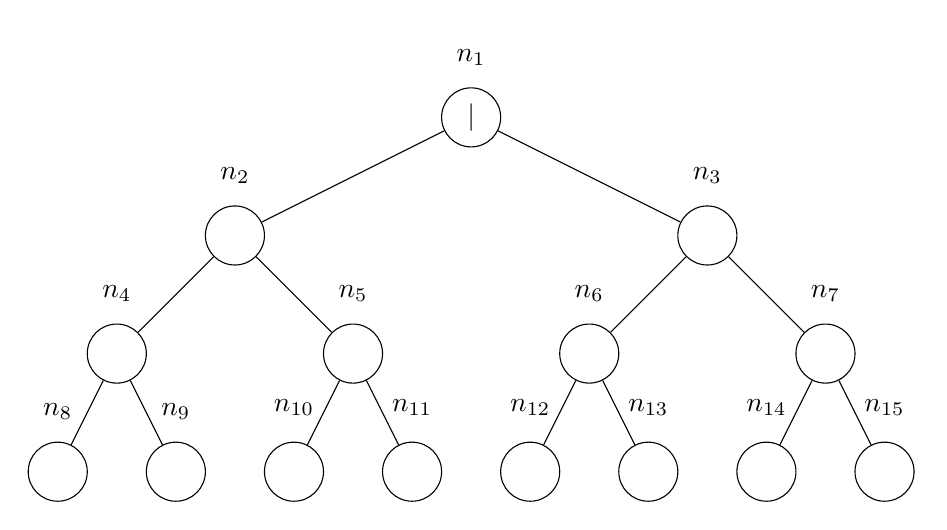
\begin{tikzpicture}[level distance=1.5cm,
level 1/.style={sibling distance=6cm},
level 2/.style={sibling distance=3cm},
level 3/.style={sibling distance=1.5cm}]
\tikzstyle{every node}=[circle,draw,minimum size=.75cm]

\node (Root) [label={\(n_1\)}] {\(|\)}
child {
    node [label={\(n_2\)}] {} 
    child {
        node [label={\(n_4\)}] {}
        child { node [label={\(n_8\)}]{} }
        child { node [label={\(n_9\)}]{} } % edge from parent node[left, draw=none] {help!}
    }
    child {
        node [label={\(n_5\)}] {}
        child { node [label={\(n_{10}\)}] {} }
        child { node [label={\(n_{11}\)}] {} }
    }
}
%
child {
    node [label={\(n_3\)}] {} 
    child {
        node [label={\(n_6\)}] {}
        child { node [label={\(n_{12}\)}]{} }
        child { node [label={\(n_{13}\)}]{} } % edge from parent node[left, draw=none] {help!}
    }
    child {
        node [label={\(n_7\)}] {}
        child { node [label={\(n_{14}\)}] {} }
        child { node [label={\(n_{15}\)}] {} }
    }
};

\end{tikzpicture}
    \caption{A part of a program which is a subtree of the original program tree. The root of this subtree has the \textit{union} operation assigned. }
    \label{fig:union-idempotent-tree}
\end{figure}{}
